Después de analizar detenidamente los requisitos se procede a detallar la solución propuesta para el desarrollo de Vihrtual-App.

\subsection{Tratamientos del dataset}

\subsection{Aspectos técnicos}
Eklegmos rasa, cumple con el capitulo anterior

\subsection{Personalidad}
caracteristicas sociales del bot, uso de emojis, efectos visuales, avatar

\subsection{Distribución}
Como web y app, facilmente accesible, no registro

\subsection{Roadmap}
Siguiendo la metodología \textit{Scrum} se propuso una ruta de desarrollo (ver figura \ref{fig:roadmap desarrollo}) centrada en la obtención de un producto mínimo via	ble lo antes posible. Para ello primeramente se realizarían los diseños del chatbot, se organizaría la información recibida y se trabajaría para la obtención de un \textit{PMI} en versión web. A partir de ese punto se publicaría una versión de prueba del \textit{bot} para con la obtención de datos reales realizar distintas iteraciones sobre el producto hasta conseguir el resultado deseado. Una vez se alcanzara el nivel de madurez requerido, la web se empaquetaría como \textit{app} para móvil y se publicaría.\\

\begin{figure}[htbp]
\centering
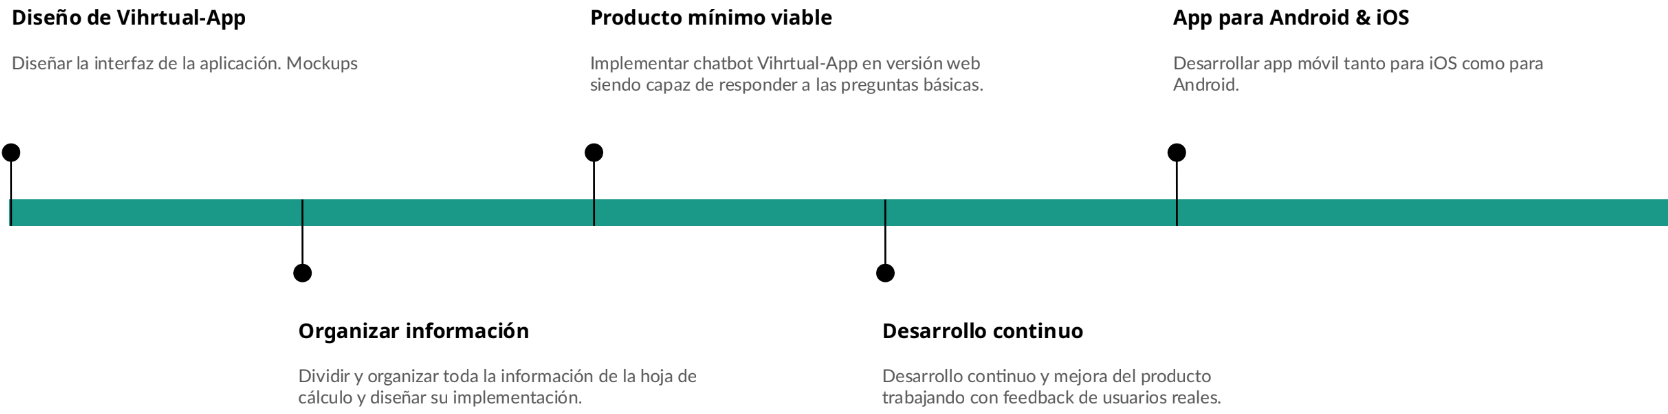
\includegraphics[scale=0.4]{../images/roadmap.png} 
\caption{\textit{Roadmap} propuesto para el desarrollo de Vihrtual-App}
\label{fig:roadmap desarrollo}
\end{figure}

Este propuesta fue presentada en una reunión con los colaboradores la Unidad de Enfermedades Infecciosas del Hospital General de Elche para obtener su aprobación. Las diapositivas se pueden encontrar en los documentos anexos a este trabajo.\\